\documentclass{article}

% if you need to pass options to natbib, use, e.g.:
% \PassOptionsToPackage{numbers, compress}{natbib}
% before loading nips_2018

% ready for submission
\usepackage[final]{nips_2018}

% to compile a preprint version, e.g., for submission to arXiv, add
% add the [preprint] option:
% \usepackage[preprint]{nips_2018}

% to compile a camera-ready version, add the [final] option, e.g.:
% \usepackage[final]{nips_2018}

% to avoid loading the natbib package, add option nonatbib:
% \usepackage[nonatbib]{nips_2018}

\usepackage[utf8]{inputenc} % allow utf-8 input
\usepackage[T1]{fontenc}    % use 8-bit T1 fonts
\usepackage{hyperref}       % hyperlinks
\usepackage{url}            % simple URL typesetting
\usepackage{booktabs}       % professional-quality tables
\usepackage{amsfonts}       % blackboard math symbols
\usepackage{nicefrac}       % compact symbols for 1/2, etc.
\usepackage{microtype}      % microtypography
\usepackage{stmaryrd}

\newcommand{\theHalgorithm}{\arabic{algorithm}}
\newcommand{\sem}[1]{\llbracket #1 \rrbracket}
\newcommand{\system}{\textsc{SCC}~}
\newcommand{\systemEnding}{\textsc{SCC}}
\newcommand{\lowerBound}{\mathscr{L}}
\newcommand{\code}[1]{{\footnotesize\texttt{#1}}}
\newcommand{\codechar}[1]{{\footnotesize{\texttt{"#1"}}}}

\usepackage{mathrsfs}
\usepackage{listings}
\usepackage{amsthm}

\usepackage{subfig} 
\usepackage{fancyvrb}


\usepackage{caption}
\usepackage{amssymb}
\usepackage{listings}
\usepackage{wrapfig}
\usepackage{tabularx}


\usepackage{verbatim}
 \usepackage{booktabs}
 % For algorithms
\usepackage{algorithm}
\usepackage{algorithmic}
\usepackage{tikz}
\usepackage{circuitikz}
\usetikzlibrary{fit,bayesnet}
\usepackage{dsfont}
\usepackage{amsmath}

\DeclareMathOperator*{\argmin}{arg\,min} % thin space, limits underneath in displays
\DeclareMathOperator*{\argmax}{arg\,max} % thin space, limits underneath in displays
 


% Packages hyperref and algorithmic misbehave sometimes.  We can fix
% this with the following command.

\newcommand{\Expect}{\mathds{E}} %{{\rm I\kern-.3em E}}
\newcommand{\indicator}{\mathds{1}} %{{\rm I\kern-.3em E}}
\newcommand{\expect}{\mathds{E}} %{{\rm I\kern-.3em E}}
\newcommand{\probability}{\mathds{P}} %{{\rm I\kern-.3em P}}

\title{Supplement to: Library Learning for Neurally-Guided Bayesian Program Induction}

% The \author macro works with any number of authors. There are two
% commands used to separate the names and addresses of multiple
% authors: \And and \AND.
%
% Using \And between authors leaves it to LaTeX to determine where to
% break the lines. Using \AND forces a line break at that point. So,
% if LaTeX puts 3 of 4 authors names on the first line, and the last
% on the second line, try using \AND instead of \And before the third
% author name.

\author{
  Kevin Ellis\\MIT\\\texttt{ellisk@mit.edu}\And Lucas Morales\\MIT\\\texttt{lucasem@mit.edu}\And Mathias Sabl\'e-Meyer\\ENS Paris-Saclay\\\texttt{mathsm@mit.edu}
  \AND
  Armando Solar-Lezama\\MIT\\\texttt{asolar@csail.mit.edu}\And Joshua B. Tenenbaum\\MIT\\\texttt{jbt@mit.edu}
  %% \And
  %% Coauthor \\
  %% Affiliation \\
  %% Address \\
  %% \texttt{email} \\
  %% \AND
  %% Coauthor \\
  %% Affiliation \\
  %% Address \\
  %% \texttt{email} \\
  %% \And
  %% Coauthor \\
  %% Affiliation \\
  %% Address \\
  %% \texttt{email} \\
  %% \And
  %% Coauthor \\
  %% Affiliation \\
  %% Address \\
  %% \texttt{email} \\
}

\begin{document}
% \nipsfinalcopy is no longer used

\maketitle

\section{An Illustration of the three steps of our algorithm}
Below we diagram the steps employed by our algorithm. At each step of the algorithm,
we have shaded the observed variables in gray and left the unobserved variables white.
Black lines correspond to a connection from the top-down
generative model, while red lines correspond to connections from the bottom-up recognition model.
\begin{figure}[h]
\centering
%  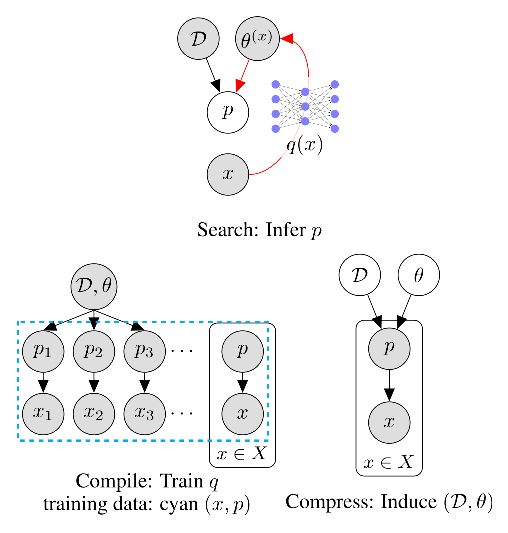
\includegraphics{figures/iterations.eps}
\begin{tikzpicture}
  \begin{scope}[shift={(2.5,0)}]
    \node[obs] at (3,3) (dx){$\mathcal{D}$};
    \node[latent] at (3.5,1.75) (zp){$p$};
    \node[obs] at (4,3) (tx){$\theta^{(x)}$};
    \node[obs] at (3.5,0.7) (xp) {$x$};
    \node[align = center] at ([yshift = -0.6cm,xshift = 0.5cm]xp.south) {Explore: Infer $p$};
    \draw [->,red] (xp.east) to[out = 0,in = 0] node(nn){} (tx.east);
    \draw [->,red] (tx) -- (zp);
    \draw [->] (dx) -- (zp);
    \node at (nn) {
      \begin{tikzpicture}[x=2.5cm,y=1.25cm,transform canvas={scale=0.2,shift={+(-1,2.5)}}]
        \tikzstyle{neuron}=[circle,fill=blue!50,minimum size=20pt]
        \fill[fill=white] (-0.25,-0.5) rectangle (2.25,-4.5);
        \node[rectangle] at (1,1) {};
        \foreach \name / \y in {1,...,4}
            \node[neuron] (I-\name) at (0,-\y) {};
        \foreach \name / \y in {1,...,3}
            \node[neuron] (H-\name) at (1,-\y-0.5) {};
        \foreach \name / \y in {1,...,4}
            \node[neuron] (O-\name) at (2,-\y) {};
        \foreach \source in {1,...,4}
            \foreach \dest in {1,...,3}
                \draw [-latex] (I-\source) -- (H-\dest);
        \foreach \source in {1,...,3}
            \foreach \dest in {1,...,4}
                \draw [-latex] (H-\source) -- (O-\dest);
      \end{tikzpicture}
    };
    \node[shift={+(0,-0.65)}] at (nn) [fill=white]{ $q(x)$ };
  \end{scope}
  \begin{scope}[shift={(0.7,-4.2)}]
    \node[obs] at (3,3) (dt){$\mathcal{D},\theta$};
    \node[obs] at ([yshift = -0.7cm,xshift = 0.0cm]dt.south) (p2){$p_2$};
    \node[obs] at ([yshift = -0.7cm,xshift = 0.0cm]p2.south) (x2){$x_2$};
    \draw [->] (p2.south) -- (x2.north);
    \draw [->] (dt.south) -- (p2.north);
    \node[obs] at ([yshift = 0cm,xshift = -0.5cm]p2.west) (p1){$p_1$};
    \node[obs] at ([yshift = -0.7cm,xshift = 0.0cm]p1.south) (x1){$x_1$};
    \draw [->] (p1.south) -- (x1.north);
    \draw [->] (dt.south) -- (p1.north);
    \node[obs] at ([yshift = 0cm,xshift = 0.5cm]p2.east) (p3){$p_3$};
    \node[obs] at ([yshift = -0.7cm,xshift = 0.0cm]p3.south) (x3){$x_3$};
    \draw [->] (p3.south) -- (x3.north);
    \draw [->] (dt.south) -- (p3.north);
    \node at ([yshift = 0cm,xshift = 0.3cm]p3.east) {$\cdots $};
    \node at ([yshift = 0cm,xshift = 0.3cm]x3.east) {$\cdots $};
      
    \node[obs] at ([yshift = 0cm,xshift = 1.3cm]p3.east) (zp){$p$};
    \node[obs] at ([yshift = 0cm,xshift = 1.3cm]x3.east) (xp) {$x$};
    \draw [->] (zp.south) -- (xp.north);
    \plate {}{(zp)(xp)}{$x\in X$};
    \draw[dashed,cyan,very thick] ([yshift = 0.5cm,xshift = -2]p1.west)
    rectangle  ([yshift = -0.45cm,xshift = +2]xp.east);
    \node[align = center] at ([yshift = -1cm,xshift = 0.6cm]x2.south) {Compile: Train $q$\\training data: cyan $(x,p)$};
  \end{scope}
    
  \begin{scope}[shift={(7.7,-4)}]
    \node[latent] at (0.5,3) (d){$\mathcal{D}$};
    \node[latent] at (1.5,3) (t){$\theta$};
    \node[obs] at (1,1.75) (z){$p$};
%     \node[latent] at (3.5,1.5) (tx){$\theta^{(x)}$};
    \node[obs] at (1,0.5) (x) {$x$};
    \edge {z}{x};
    \edge {d,t}{z};
    \plate {}{(z)(x)}{$x\in X$};
    \node[align = center] at ([yshift = -1cm]x.south) {Compress: Induce $(\mathcal{D},\theta)$};
  \end{scope}
\end{tikzpicture}
\end{figure}

\section{Program Representation}\label{programrepresentation}
We choose to represent programs using $\lambda$-calculus~\cite{pierce}.
A $\lambda$-calculus expression is either:
\begin{itemize}
  \item[--] A \emph{primitive}, like the number 5 or the function \texttt{sum}.
  \item[--] A \emph{variable}, like $x$, $y$, or $z$.
  \item[--] A $\lambda$\emph{-abstraction}, which creates a new function.  $\lambda$-abstractions have a variable and a body. The body is a $\lambda$-calculus expression. Abstractions are written as $\lambda \text{var}. \text{body}$ or in Lisp syntax as \mbox{\texttt{(lambda (\textrm{var}) \textrm{body})}}.
  \item[--] An \emph{application} of a function to an argument. Both the function and the argument are $\lambda$-calculus expressions. The application of the function $f$ to the argument $x$ is written as $f\; x$ or as \texttt{($f$ x)}.
\end{itemize}

For example, the function which squares the logarithm of a number is
$\lambda x.\text{\tt(square (log $x$))}$, and the identity function $f(x) = x$ is $\lambda x.x$. The
$\lambda$-calculus serves as a spartan but expressive Turing complete
program representation, and distills the essential features of functional
programming languages like Lisp.

However, many $\lambda$-calculus expressions correspond to ill-typed programs, such as the program that takes the logarithm of the Boolean \texttt{true} (i.e., \texttt{log true}) or which applies the number five to the identity function
(i.e., $5 \; (\lambda x.x)$).
We use a well-established typing system for $\lambda$-calculus called \emph{Hindley-Milner typing}~\cite{pierce}, which is used in programming languages like OCaml.
The purpose of the typing system is to ensure that our programs never call a function with a type it is not expecting (like trying to take the logarithm of \texttt{true}).
Hindley-Milner has two important features:
Feature 1: It supports \emph{parametric polymorphism}, meaning that types can have variables in them, called \emph{type variables}. Lowercase Greek letters are conventionally used for  type variables.
For example, the type of the identity function is $\alpha\to\alpha$, meaning it takes something of type $\alpha$ and return something of type $\alpha$. A function that returns the first element of a list has the type $[\alpha]\to\alpha$. Type variables are not the same as variables introduced by $\lambda$-abstractions.
Feature 2: Remarkably, there is a  simple algorithm for automatically inferring the polymorphic Hindley-Milner type of a $\lambda$-calculus expression~\cite{damas1982principal}.
Our generative model over programs performs Hindley-Milner type inference during sampling:
\emph{Unify} in the generative model uses the machinery of Hindley-Milner to
ensure that the generated programs have valid polymorphic types.
A satisfactory exposition of Hindley-Milner is beyond the scope of this paper,
but~\cite{pierce} offers a nice overview of lambda calculus and typing systems like Hindley-Milner.

%% \begin{figure}
%%   \begin{align}
%%     \text{primitive types} & 
%%     \end{align}
%%   \end{figure}

\vfill
\section{Generative model over programs}

Alg.~\ref{programGenerativeModel} is a procedure for drawing
samples from the generative model $(\mathcal{D},\theta)$.  In practice, we
enumerate programs in order of their probability under  Alg.~\ref{programGenerativeModel} rather than sample them.

\begin{figure}[H]
  \centering
  \begin{minipage}{0.5\textwidth}    
    \begin{algorithm}[H]
       \caption{Generative model over programs}
       \label{programGenerativeModel}
       \begin{algorithmic}
    %%      \STATE \textbf{function} sampleProgramFromDSL$(\mathcal{D}, \theta, \tau)$:
    %%   \STATE {\bfseries Input:} DSL $\mathcal{D}$, weight vector $\theta$, type $\tau$
    %%   \STATE \textbf{Output:} a program whose type unifies with $\tau$
    %%   \STATE \textbf{return} sample$(\mathcal{D}, \theta, \varnothing, \tau)$
    %% \STATE
         \STATE \textbf{function} sample$(\mathcal{D}, \theta, \mathcal{E}, \tau)$:
      \STATE {\bfseries Input:} DSL $(\mathcal{D},\theta)$, environment $\mathcal{E}$, type $\tau$
      \STATE \textbf{Output:} a program whose type unifies with $\tau$
      \IF{$\tau = \alpha\to\beta$}
      \STATE var $\gets$ an unused variable name
      \STATE body $\sim$ sample$(\mathcal{D},\theta,\{\text{var}:\alpha\}\cup\mathcal{E},\beta)$
       \STATE \textbf{return} \code{(lambda (}var\code{) }body\code{)}
       \ENDIF
       %   \ELSE
       \STATE $\text{primitives} \gets\{p | p: \tau' \in \mathcal{D}\cup\mathcal{E}$ \\
          \hspace*{6.9em}$\text{if }\tau\text{ can unify with yield}(\tau') \} $
       
       \STATE Draw $e\sim \text{primitives}$, w.p. $\propto\theta_e$ if $e\in \mathcal{D}$ \\
          \hspace*{8.8em}w.p. $\propto\frac{\theta_{var}}{|\text{variables}|}$ if $e\in \mathcal{E}$
       \STATE Unify $\tau$ with yield$(\tau')$.
       \STATE $\left\{\alpha_k \right\}_{k = 1}^K\gets\text{args}(\tau')$ 
    %   \STATE unify$(\tau,\beta)$
       \FOR{$k=1$ {\bfseries to} $K$}
     \STATE $a_k\sim\text{sample}(\mathcal{D},\theta,\mathcal{E},\alpha_k)$
     \ENDFOR
     \STATE \textbf{return} \code{(}$e\;a_1\; a_2\; \cdots\; a_K$\code{)}
     \STATE\textbf{where:}
     \STATE yield$(\tau) = \begin{cases}
       \text{yield}(\beta)   &\text{ if }\tau = \alpha\to \beta\\
       \tau   &\text{ otherwise.}
     \end{cases}$ 
     \STATE  args$(\tau) = \begin{cases}
       [\alpha] + \text{args}(\beta)   &\text{ if }\tau = \alpha\to \beta\\
       []   &\text{ otherwise.}
     \end{cases}$
    \end{algorithmic}
    \end{algorithm}
  \end{minipage}
\end{figure}


\section{Neural Recognition Model Architecture}

The neural recognition model regresses from an observation (set of input/output pairs: $\left\{(i_n,o_n) \right\}_{n\leq N}$) to a $|\mathcal{D}| + 1$ dimensional vector. Each input/output pair is processed by an identical encoder network;
the outputs of the encoders are average and passed to an MLP with 1 hidden layer, 32 hidden units, and a ReLU activation:
\begin{align}
  q(x) = \text{MLP}\left(\text{Average}\left(\left\{\text{encoder}\left(i_n,o_n \right) \right\}_{n\leq N} \right) \right)
\end{align}



For the string editing and list domains,
the inputs and outputs are sequences. Our encoder for these domains is a bidirectional GRU with 64 hidden units that reads each input/output pair; we concatenate the input and output along with a special delimiter
symbol between them.
We MaxPool the final hidden unit activations in the GRU along both passes of the bidirectional GRU.

For symbolic regression,
the input/outputs are densely sampled points along the curve of the function.
We rendered these points to a graph,
and pass the image of the graph to a convolutional network,
which acts as the encoder.

\section{DSL Induction}

\subsection{Fragment grammars}

`Fragment grammars'~\cite{tim} is a formalism from computational linguistics
developed for the purpose of modeling
the reuse of structure
in natural language.
Here,
we will adapt the fragment grammar formalism
to model the reuse of structure in
a formal language ($\lambda$ calculus),
interpreting reuse of structure as subroutines.

In the original fragment grammar formalism,
a fragment grammar
contains a probabilistic CFG called its \emph{base grammar};
a \emph{fragment} is a tree drawn from the base grammar,
but which can contain nonterminal symbols.
As a motivating example,
consider the following base grammar:
\begin{align*}
  S\to&(+ \;S\; S)\\
  S\to&(\times \;S  \;S)\\
  S\to&0\\
      S\to&1  
\end{align*}
An example expression drawn from this grammar is $(+ \;1\; (\times \;0 \;0))$.
An example \emph{fragment} drawn from this grammar $(+ \;1\; (\times \;S\; S))$.

When extending fragment grammars to $\lambda$-calculus we write nonterminal symbols as free variables,
and use the (current) DSL as our base grammar.
For example, if our DSL includes addition, multiplication, and the numbers zero \& one (as in our example base grammar),
then a possible  $\lambda$-fragment would be $(+ \;1\; (\times \;x\; y))$.

In order to use fragments
for DSL induction,
we need several
pieces: (1) a procedure for proposing fragments from programs found in the frontiers (described in figure~\ref{extractFragments});
(2) a procedure for evaluating
the likelihood of a program given that a fragment
has been added to the DSL (defined in figure~\ref{match});
and (3) a procedure for converting a fragment to a subroutine (i.e., a closed, typed $\lambda$-calculus expression; described in Figure~\ref{close}).
Putting these procedures together, Algorithm~\ref{grammarInductionAlgorithm}
is used to induce a new DSL.

%\vfill\pagebreak
\begin{figure}  
  \begin{minipage}[c]{\textwidth}\toprule 
    \begin{align*}
  \text{fragments}(\lambda z.e)& = \text{fragments}'(\lambda z.e)\cup \text{fragments}(e)\\
  \text{fragments}(f \; x)& = \text{fragments}'(f \; x)\cup \text{fragments}(f)\cup\text{fragments}(x)\\
  \text{fragments}(e)& = \varnothing\text{, if $e$ is a variable or primitive.}\\
  \\
  \text{fragments}'(\lambda z.e)& = \left\{\lambda z.e' | e'\in \text{fragments}'(e) \right\}\cup \left\{v \right\}\text{, $v$ a free variable}\\
  \text{fragments}'(f\; x)& = \left\{f'\; x' | f'\in \text{fragments}'(f),\;x'\in \text{fragments}'(x) \right\}\cup \left\{v \right\}\text{, $v$ a free variable}\\
    \text{fragments}'(e)& = \left\{e\right\}\cup \left\{v \right\}\text{, $v$ a free variable, $e$ a variable or primitive}
\end{align*}\bottomrule 
    \end{minipage}
\caption{Procedure for extracting possible fragments from a program. To prevent an explosion in the number of fragments, we also cap the number of free variables in a fragment to 3.}\label{extractFragments}
\end{figure}
\begin{figure}
  \toprule \begin{minipage}[c]{\textwidth}
    \begin{align*}
      \text{closeFragment}(e)& = \text{closeFragment}(\lambda z.e)\text{, if $z$ is a free variable in $e$}\\
      \text{closeFragment}(e)& = e\text{, if $e$ has no free variables.}
    \end{align*}
    \bottomrule 
  \end{minipage}
  \caption{Procedure for converting a fragment to a subroutine.}\label{close}
\end{figure}

\begin{figure}
  \toprule \begin{minipage}[c]{\textwidth}
    \begin{align*}
      \probability[p|\mathcal{D},\theta]& = P_{\mathcal{D},\theta} (p|\tau,\varnothing )\text{, where $p:\tau$}\\
      P_{\mathcal{D},\theta} (\lambda z.p|\alpha\to\beta,\mathcal{E})& =
      P_{\mathcal{D},\theta}(p|\beta,[\tau\mapsto\alpha]\mathcal{E})\text{, where $\tau$ a fresh type variable}\\
      P_{\mathcal{D},\theta}(e|\tau,\mathcal{E})& = \underbrace{\sum_{f,xs\in \text{parse}(e)} P'_{\mathcal{D},\theta}(f,xs|\tau,\mathcal{E})}_{\text{Marginalizing out how $\mathcal{D}$ produced $e$}}\text{, when $e$ not a $\lambda$-abstraction}\\
      \\
      P'_{\mathcal{D},\theta}(f,xs|\tau,\mathcal{E})& = \underbrace{\sum_{f':\tau_1\to\tau_2\to\cdots\to\tau\in \mathcal{D}}\frac{\theta_f}{Z_{\tau,\mathcal{D},\theta,\mathcal{E}}}
        \indicator[\text{match}(f',f)\not=\bot]}_{\text{Marginalize over which fragment produced $f,xs$}}\times\\&\prod_{n=1}^{|xs|}P_{\mathcal{D},\theta}(x_n|\tau_n,\mathcal{E})\prod_{e,\tau'\in \text{match}(f',f)}P_{\mathcal{D},\theta}(e|\tau',\mathcal{E})\\
      \\
      \text{match}(\lambda z.b,\lambda z.b')& = \text{match}(b,b')\\
      \text{match}(f\;x,f'\;x')& = \text{match}(f,f')\cup\text{match}(x,x')\\
      \text{match}(p,p)& = \varnothing \text{, $p$ a primitive or variable bound in fragment}\\
      \text{match}(v,p)& = \left\{v\mapsto p   \right\} \text{, $v$ a variable free in fragment, $p$ not containing free variables bound in fragment}\\
      \text{match}(e,e')& = \bot\text{, otherwise.}
      \\
      \\
      Z_{\tau,\mathcal{D},\theta,\mathcal{E}}& = \underbrace{\sum_{f:\tau_1\to\tau_2\to\cdots\to\tau\in \mathcal{D}\cup\mathcal{E}}\theta_f}_{\text{Normalizing constant for type $\tau$}}\\\\
      \text{parse}(f\;x)& = \left\{f',xs+[x] \;|\; f',xs\in \text{parse}(f) \right\}\cup\left\{f\;x \right\}\\
      \text{parse}(e)& = \left\{e,[] \right\} \text{, $e$ not an application}
    \end{align*}
  \end{minipage}
  \bottomrule
  \caption{Procedure for calculating likelihood of a program after a new fragment has been added to the DSL. For simplicity we omit typing context and reuse type variables to indicate unification, as is commonly done in e.g. Prolog.}\label{match}
  \end{figure}




\begin{figure}[H]
  \centering
  \begin{minipage}{\textwidth}    
    \begin{algorithm}[H]
    \setcounter{algorithm}{2} % there are two algorithms in the main paper.
       \caption{DSL Induction Algorithm}
       \label{grammarInductionAlgorithm}
       \begin{algorithmic}
         \STATE {\bfseries Input:} Set of frontiers $\{\mathcal{F}_x\}$
         \STATE \textbf{Hyperparameters:} Pseudocounts $\alpha$, regularization parameter $\lambda$
         \STATE \textbf{Output:} DSL $\mathcal{D}$, weight vector $\theta$
         \STATE Define $L(\mathcal{D},\theta) =  \prod_x \sum_{p\in \mathcal{F}_x} \probability[p|\mathcal{D},\theta]$
         \STATE Define $\theta^*(\mathcal{D}) = \argmax_\theta \text{Dir}(\theta|\alpha) L(\mathcal{D},\theta)$
         \STATE Define $\text{score}(\mathcal{D}) = \log \probability[\mathcal{D}] + L(\mathcal{D},\theta^*) - \|\theta\|_0$
         \STATE $\mathcal{D}\gets$ every primitive in $\{\mathcal{F}_x\}$
         \WHILE {true}
         \STATE N $\gets \{\mathcal{D}\cup \{s\} | x\in X, p\in \mathcal{F}_x, s\in \text{fragments}(p)\}$
         \STATE $\mathcal{D}'\gets \argmax_{\mathcal{D}'\in N}\text{score}(\mathcal{D}') $
         \STATE \textbf{if }$\text{score}(\mathcal{D}') < \text{score}(\mathcal{D})$\textbf{ return }$\left\{\text{closeFragment}(s)|s\in \mathcal{D} \right\},\theta^*(\mathcal{D})$
         \STATE $\mathcal{D}\gets\mathcal{D}'$
         \ENDWHILE
       \end{algorithmic}
    \end{algorithm}
  \end{minipage}
\end{figure}

\subsection{Estimating $\theta$}

We use an EM algorithm to estimate the continuous parameters of the DSL, e.g. $\theta$.
Suppressing dependencies on $\mathcal{D}$, the EM updates are
\begin{align}
\label{maximizeStep}  \theta& = \argmax_\theta \log P(\theta) + \sum_x \expect_{Q_x}\left[\log \probability\left[p|\theta \right] \right]\\
  Q_x(p)&\propto \probability[x|p]\probability[p|\theta]
  \end{align}
In the M step of EM we will update $\theta$ by instead maximizing a lower bound on $\log \probability[p|\theta]$,
making our approach an instance of Generalized EM.

We write $c(e,p)$ to mean the number of times that primitive $e$ was used in program $p$; $c(p)= \sum_{e\in \mathcal{D}}c(e,p)$ to mean the total number of primitives used in program $p$; $R(p)$ to mean the sequence of types input to sample in Alg.~1 of the main paper. Jensen's inequality gives a lower bound on the likelihood:
\begin{align*}
  &\sum_x\expect_{Q_x}\left[  \log \probability[p|\theta] \right] =\\
  &\sum_{e\in \mathcal{D}} \log \theta_e \sum_x\expect\left[c(e,p_x) \right] -
  \sum_\tau\expect\left[\sum_x c(\tau,p_x)  \right]\log \sum_{\substack{e:\tau'\in \mathcal{D}\\\text{unify}(\tau,\tau')}}\theta_e  \\
 =   &\sum_e C(e)\log \theta_e  - \beta\sum_\tau\frac{\expect\left[\sum_x c(\tau,p_x)  \right]}{\beta}\log \sum_{\substack{e:\tau'\in \mathcal{D}\\\text{unify}(\tau,\tau')}}\theta_e  \\
 \geq    &\sum_e C(e)\log \theta_e  - \beta\log \sum_\tau\frac{\expect\left[\sum_x c(\tau,p_x)  \right]}{\beta}\sum_{\substack{e:\tau'\in \mathcal{D}\\\text{unify}(\tau,\tau')}}\theta_e  \\
     =     &\sum_e C(e)\log \theta_e  - \beta\log \sum_\tau\frac{R(\tau)}{\beta}\sum_{\substack{e:\tau'\in \mathcal{D}\\\text{unify}(\tau,\tau')}}\theta_e  
  %% &\geq\sum_{e\in \mathcal{D}} c(e,p)\log \theta_e - c(p)\log \frac{1}{c(p)}\sum_{\tau\in R(p)} \sum_{\substack{e:\tau'\in \mathcal{D}\\\text{unify}(\tau,\tau')}}\theta_e\\
  %% & = \sum_{e\in \mathcal{D}} c(e,p)\log \theta_e - c(p)\log\frac{1}{c(p)} \sum_{e\in \mathcal{D}} r(e,p)\theta_e
\end{align*}
where we have defined
\begin{align*}
  C(e)&\triangleq  \sum_x\expect\left[c(e,p_x) \right]\\
  R(\tau)&\triangleq \expect\left[\sum_x c(\tau,p_x)  \right]\\
  \beta&\triangleq\sum_\tau \expect\left[\sum_x c(\tau,p_x)  \right]
\end{align*}
Crucially it was defining $\beta$ that let us use Jensen's inequality. 
Recalling from the main paper that $P(\theta)\triangleq\text{Dir}(\alpha)$,
we have the following lower bound on M-step objective:
\begin{align}
\sum_e (C(e) + \alpha)\log \theta_e  - \beta\log \sum_\tau\frac{R(\tau)}{\beta}\sum_{\substack{e:\tau'\in \mathcal{D}\\\text{unify}(\tau,\tau')}}\theta_e    
\end{align}
Differentiate with respect to $\theta_e$, where $e:\tau$, and set to zero to obtain:
\begin{align}
  &  \frac{C(e) + \alpha}{\theta_e}\propto\sum_{\tau'}\indicator\left[\text{unify}(\tau,\tau') \right] R(\tau')\\
&  \theta_e\propto\frac{C(e) + \alpha}{\sum_{\tau'}\indicator\left[\text{unify}(\tau,\tau') \right] R(\tau')}
\end{align}
The above is our estimator for $\theta_e$.
Despite the convoluted derivation, the above estimator has an intuitive interpretation.
The quantity $C(e)$ is the expected number of times that we used $e$.
The quantity $\sum_{\tau'}\indicator\left[\text{unify}(\tau,\tau') \right] R(\tau')$
is the expected number of times that we \emph{could have} used $e$.
The hyperparameter $\alpha$ acts as pseudocounts that are
added to the number of times that we used each primitive,
and are not added to the number of times that we could have used each primitive.


We are only maximizing a lower bound on the log posterior; when is this lower bound tight?
This lower bound is tight whenever all
of the types of the expressions in the DSL are not polymorphic, in which case our DSL is equivalent to a PCFG
and this estimator is equivalent to the inside/outside algorithm.
Polymorphism introduces context-sensitivity to the DSL,
and exactly maximizing the likelihood with respect to $\theta$
becomes intractable,
so for domains with polymorphic types we use this estimator.

\begin{comment}
\section{Initial Domain-Specific Languages}
\subsection{Boolean Circuits}
\begin{center}
\tt
\begin{tabular}{| l | l |}
  \hline
  \textrm{\emph{name}} & \textrm{\emph{type}} \\
  \hline
    nand & $\text{bool}\to \text{bool}\to \text{bool}$ \\  \hline
\end{tabular}
\end{center}

\subsection{Symbolic Regression}
\begin{center}
\tt
\begin{tabular}{| l | l |}
  \hline
  \textrm{\emph{name}} & \textrm{\emph{type}} \\
  \hline
  + & $\mathbb{R}\to \mathbb{R}\to \mathbb{R}$ \\
  *&  $\mathbb{R}\to \mathbb{R}\to \mathbb{R}$\\
  real&$\mathbb{R}$\\\hline
\end{tabular}
\end{center}


\subsection{String Editing}
\begin{center}
\tt
\begin{tabular}{| l | l |}
  \hline
  \textrm{\emph{name}} & \textrm{\emph{type}} \\
  \hline
  0&$\mathbb{Z}$\\
  +1&$\mathbb{Z}\to \mathbb{Z}$\\
  -1&$\mathbb{Z}\to \mathbb{Z}$\\
  split&$\text{char}\to \text{string}\to \left[\text{string} \right]$\\
  join&$\text{string}\to \left[\text{string} \right]\to \text{string}$\\
  map&$(\text{string}\to \text{string})$\\
  &$\qquad\quad\to\left[\text{string} \right]\to \left[\text{string} \right]$\\
  nth&$\mathbb{Z}\to \left[\text{string} \right]\to \text{string}$\\
  slice&$\mathbb{Z}\to \mathbb{Z}\to \text{string}\to \text{string}$\\
  length&$\text{string}\to \mathbb{Z}$\\
  ""&string\\
  ","\quad" "&char\\
  "<"\quad">" &char \\
  chr->str&$\text{char}\to \text{string}$\\
  trim&$\text{string}\to \text{string}$\\
  upper&$\text{string}\to \text{string}$\\
  lower&$\text{string}\to \text{string}$\\
  capitalize&$\text{string}\to \text{string}$\\\hline
\end{tabular}
\end{center}


\vfill


\subsection{List Functions}
The lower section with seven primitives designates those given to the
\emph{rich} DSL variant and not the \emph{base} variant. The rich variant is
not supplied the \texttt{if} primitive, because its primary intention is to
enable the learning of the lower five concepts.
Greek letters represent polymorphic types.
\begin{center}
\tt
\begin{tabular}{| l | l |}
  \hline
  \textrm{\emph{name}} & \textrm{\emph{type}} \\
  \hline
    empty & $\left[\alpha\right]$ \\
    singleton & $\alpha \to \left[\alpha\right]$ \\
    concat & $\left[\alpha\right] \to \left[\alpha\right] \to \left[\alpha\right]$ \\
    mapi & $(\mathbb{Z} \to \alpha \to \beta)$ \\
    & \qquad\qquad$\to \left[\alpha\right] \to \left[\beta\right]$ \\
    reducei & $(\beta \to \mathbb{Z} \to \alpha \to \beta)$\\
    & \qquad\qquad$\to \beta \to \left[\alpha\right] \to \beta$ \\
    \hline
    if & bool $\to \alpha \to \alpha \to \alpha$ \\
    \hline
    true & bool \\
    not & bool $\to$ bool \\
%UNUSED+UNNECESSARY:    and & bool $\to$ bool $\to$ bool \\
%UNUSED+UNNECESSARY:    or & bool $\to$ bool $\to$ bool \\
    0 $\cdots$ 5 & $\mathbb{Z}$ \\
    + & $\mathbb{Z} \to \mathbb{Z} \to \mathbb{Z}$ \\
    * & $\mathbb{Z} \to \mathbb{Z} \to \mathbb{Z}$ \\
    negate & $\mathbb{Z} \to \mathbb{Z}$ \\
    mod & $\mathbb{Z} \to \mathbb{Z} \to \mathbb{Z}$ \\
    eq? & $\mathbb{Z} \to \mathbb{Z} \to$ bool \\
    gt? & $\mathbb{Z} \to \mathbb{Z} \to$ bool \\
    is-prime & $\mathbb{Z} \to$ bool \\
    is-square & $\mathbb{Z} \to$ bool \\
    range & $\mathbb{Z} \to$ [$\mathbb{Z}$] \\
    sort & $\left[\mathbb{Z}\right] \to \left[\mathbb{Z}\right]$ \\
    \hline
    sum & $\left[\mathbb{Z}\right] \to \mathbb{Z}$ \\
    reverse & $\left[\alpha\right] \to \left[\alpha\right]$ \\
    all & $(\alpha \to$ bool$) \to \left[\alpha\right] \to$ bool \\
    any & $(\alpha \to$ bool$) \to \left[\alpha\right] \to$ bool \\
    index & $\mathbb{Z} \to \left[\alpha\right] \to \alpha$ \\
    filter & $(\alpha \to$ bool$) \to \left[\alpha\right] \to \left[\alpha\right]$ \\
    slice & $\mathbb{Z} \to \mathbb{Z} \to \left[\alpha\right] \to \left[\alpha\right]$ \\
  \hline
\end{tabular}
\end{center}
  \end{comment}

\section{Hyperparameters \& Implementation Details}
We set structure penalty $\lambda = 1$ (Eq.~5 of the main paper) and
smoothness parameter $\alpha = 10$ (Eq.~6 of the main paper)
for all experiments.
For list processing and text editing we used a search timeout of two hours;
because the symbolic regression problems are easier,
we used a timeout of only five minutes for these.


Because the frontiers can become very large in later iterations of the algorithm,
we only keep around the top $10^4$ programs in the frontier $\mathcal{F}_x$ as measured by $\probability[x,p|\mathcal{D},\theta]$.




\section{Why not the ELBO Bound?}

Our lower bound $\lowerBound$ is unconventional,
and one might wonder why we do not instead maximize an ELBO-style bound like in a VAE or in the EM algorithm.
Surprisingly, maximizing an ELBO-style bound
leads to a pathological behavior that  causes the model to easily become trapped in local optima.


If we were to maximize the ELBO bound to perform inference in
our generative model,
then, during DSL induction, we would seek a new $(\mathcal{D}^*,\theta^*)$ maximizing the following lower bound on the likelihood (along with an unimportant regularizing term on the DSL):
\begin{align}
  &  \sum_{x\in X}\expect_{p\sim Q_x}\left[\log \probability[p|\mathcal{D}^*,\theta^*] \right] \label{EM}\\
  & Q_x(p)\triangleq \probability[p|x,\mathcal{D},\theta]
\end{align}
where $(\mathcal{D},\theta)$ is our current estimate of the generative
model.  These equations fall out of an EM-style derivation, and one
could replace $Q_x(p)$ with the recognition model $q(p|x)$, either
using importance sampling (so the expectation in Eq.~\ref{EM} is taken
over $q$ and we reweigh using $Q_x$) or by directly using $q$ as our approximate posterior over the program that solves task $x$.

We do not maximize a bound of this form because it
takes an expectation over the \emph{previous} iteration's
posterior over programs,
so the approximate posterior $Q_x$ at the next iteration
ends up being very close to previous approximate posterior.
Intuitively,
we want the DSL induction to be a function \emph{only} of the programs that we have found,
and \emph{not} be a function of how the previous generative model weighed them.
In practice,
we found that maximizing EM-style bounds, like the ELBO,
leads to a kind of hysteresis effect,
where the next generative model too closely matches the previous one,
causing the algorithm to easily become trapped in local optima.

\begin{comment}
b
\section{Example String Editing Tasks}



We automatically generated 600 string editing problems split 75/25 train/test.
The following are representative problems:


\begin{center}
\begin{tabular}{|l|l|}
  \hline Input&Output\\
  \hline\multicolumn{2}{|c|}{Double}\\
  \hline
vlxS & vlxSvlxS \\
 JkVC & JkVCJkVC \\
 dbxD & dbxDdbxD \\
 gQgB & gQgBgQgB \\
  \hline\multicolumn{2}{|c|}{Extract string delimited by ',' (inclusive),' '}\\
  \hline
LsR,uhMZI wIL & ,uhMZI  \\
 tMY,KdF hhT & ,KdF  \\
 UUPdC,UAd kCgtq & ,UAd  \\
 gQgGN,VMJ FjrXZ & ,VMJ \\
  \hline\multicolumn{2}{|c|}{Apply first 2 characters to input delimited by '.'}\\
  \hline
OhCQN.DlH.LdkJ.pLh & OhDlLdpL \\
 CZr.mveZr.dvjP.YMJpg & CZmvdvYM \\
 bpub.VkkZ.dYdPr & bpVkdY \\
 zjNA.wFwY.WMMqh.OFdbr & zjwFWMOF \\
  \hline\multicolumn{2}{|c|}{Apply first 2 characters to string delimited by ' ','.'}\\
  \hline
fNA YWyL.JDD & YW \\
 YWozt TPW.nczz & TP \\
 RJwiT dpW.uFU & dp \\
 FTp gNMo.JsZB & gN \\
  \hline\multicolumn{2}{|c|}{Apply strip to string delimited by ',','.'}\\
  \hline
iNEP,  GigW .Xlm & GigW \\
 xhpH,  QvwnW .mfK & QvwnW \\
 weWIC,IQjhWa .fGKz & IQjhWa \\
 xZUm, FpdE.ETcr & FpdE \\
  \hline\multicolumn{2}{|c|}{Drop first character}\\
  \hline
WYPvm & YPvm \\
 terHk & erHk \\
 asWM & sWM \\
 tBdT & BdT \\
\hline
\end{tabular}
\end{center}
\end{comment}

\section{List Processing Data Set}
Each list processing tasks we created is in described in
Tbl~\ref{listdataset}.

\begin{table}[h]
  \centering\footnotesize
  \begin{tabular}{|l|l|}\hline
    add-k for k $\in\{0..5\}$&
kth-largest for k $\in\{1..5\}$\\
    append-index-k for k $\in\{1..5\}$&
kth-smallest for k $\in\{1..5\}$\\
    append-k for k $\in\{0..5\}$&
last\\
    bool-identify-geq-k for k $\in\{0..5\}$&
len\\
    bool-identify-is-mod-k for k $\in\{1..5\}$&
max\\
    bool-identify-is-prime&
min\\
    bool-identify-k for k $\in\{0..5\}$&
modulo-k for k $\in\{1..5\}$\\
    caesar-cipher-k-modulo-n&
mult-k for k $\in\{0..5\}$\\
    \qquad for k $\in\{0..5\}$ and n $\in\{1..5\}$&
odds\\
    count-head-in-tail&
pop\\
    count-k for k $\in\{0..5\}$&
pow-k for k $\in\{1..5\}$\\
    drop-k for k $\in\{0..5\}$&
prepend-index-k for k $\in\{1..5\}$\\
    dup&
prepend-k for k $\in\{0..5\}$\\
    empty&
product\\
    evens&
range\\
    fibonacci&
remove-empty-lists\\
    has-head-in-tail&
remove-eq-k for k $\in\{0..3\}$\\
    has-k for k $\in\{0..5\}$&
remove-gt-k for k $\in\{0..3\}$\\
    head&
remove-index-k for k $\in\{1..5\}$\\
    index-head&
remove-mod-head\\
    index-k for k $\in\{1..5\}$&
remove-mod-k for k $\in\{2..5\}$\\
    is-evens&
repeat\\
    is-mod-k for k $\in\{1..5\}$&
repeat-k for k $\in\{1..5\}$\\
    is-odds&
repeat-many\\
    is-primes&
replace-all-with-index-k for k $\in\{1..5\}$\\
    is-squares&
reverse\\
    keep-eq-k for k $\in\{0..3\}$&
rotate-k for k $\in\{1..5\}$\\
    keep-gt-k for k $\in\{0..3\}$&
slice-k-n for k $\in\{1..5\}$ and n $\in\{1..5\}$\\
    keep-mod-head&
sort\\
    keep-mod-k for k $\in\{1..5\}$&
sum\\
    keep-primes&
tail\\
    keep-squares&
take-k for k $\in\{1..5\}$\\
\hline
  \end{tabular}
  \normalsize
  ~\\~\\\caption{Our list processing data set}\label{listdataset}
\end{table}

\section{Learned DSLs}

Here we present representative DSLs learned by our model. DSL primitives
discovered by the algorithm are prefixed with \lstinline!#!.
Variables are prefixed with \lstinline!$!, and we adopt De Bruijn indices to
model bound variables~\cite{pierce}.

\onecolumn

\lstset{
  basicstyle=\footnotesize,
  escapechar=@,
  breaklines=true,
  breakatwhitespace=true,
  postbreak=\mbox{\textcolor{red}{$\hookrightarrow$}\space}
}

\subsection{List processing}
\begin{lstlisting}
#(+ 1 1)
#(@$\lambda$@ (cdr (cdr $0)))
#(@$\lambda$@ (foldr $0 1 (@$\lambda$@ (@$\lambda$@ (* $0 $1)))))
#(@$\lambda$@ (cons (car $0) nil))
#(@$\lambda$@ (@$\lambda$@ (foldr $0 $1 (@$\lambda$@ (@$\lambda$@ (cons $1 $0))))))
#(@$\lambda$@ (@$\lambda$@ (foldr $0 (is-nil $0) (@$\lambda$@ (@$\lambda$@ (if $0 $0 (eq? $3 $1)))))))
#(@$\lambda$@ (map (@$\lambda$@ (eq? $1 $0))))
#(@$\lambda$@ (* $0 (* $0 $0)))
#(+ 1 #(+ 1 1))
#(@$\lambda$@ (map (@$\lambda$@ (gt? $0 $1))))
#(@$\lambda$@ (foldr $0 nil (@$\lambda$@ (@$\lambda$@ (if (is-square $1) (cons $1 $0) $0)))))
#(@$\lambda$@ (map (@$\lambda$@ (eq? $0 (length (range $0)))) $0))
#(@$\lambda$@ (@$\lambda$@ (map (@$\lambda$@ (index $0 $1)) (range $1))))
#(@$\lambda$@ (cdr (#(@$\lambda$@ (cdr (cdr $0))) $0)))
#(@$\lambda$@ (map (@$\lambda$@ (index 1 $1))))
#(@$\lambda$@ (foldr $0 nil (@$\lambda$@ (@$\lambda$@ (cons $1 (cons $1 $0))))))
#(@$\lambda$@ (@$\lambda$@ (cons (car $0) $1)))
#(+ 1 #(+ 1 #(+ 1 1)))
#(@$\lambda$@ (map (@$\lambda$@ (gt? 1 (mod $0 $1)))))
#(@$\lambda$@ (@$\lambda$@ (map (@$\lambda$@ (mod (+ $0 $1) $2)))))
#(@$\lambda$@ (#(@$\lambda$@ (@$\lambda$@ (foldr $0 $1 (@$\lambda$@ (@$\lambda$@ (cons $1 $0)))))) (#(@$\lambda$@ (@$\lambda$@ (foldr $0 $1 (@$\lambda$@ (@$\lambda$@ (cons $1 $0)))))) $0 $0) $0))
#(@$\lambda$@ (@$\lambda$@ (#(@$\lambda$@ (@$\lambda$@ (foldr $0 $1 (@$\lambda$@ (@$\lambda$@ (cons $1 $0)))))) (cons $0 nil) $1)))
#(+ #(+ 1 #(+ 1 1)) #(+ 1 1))
#(@$\lambda$@ (map (@$\lambda$@ (+ #(+ 1 #(+ 1 1)) (+ $1 $0)))))
#(@$\lambda$@ (map (@$\lambda$@ (+ $0 $1))))
#(@$\lambda$@ (@$\lambda$@ (foldr $0 (is-nil $0) (@$\lambda$@ (@$\lambda$@ (gt? $1 (#(@$\lambda$@ (* $0 (* $0 $0))) $3)))))))
#(@$\lambda$@ (foldr $0 0 (@$\lambda$@ (@$\lambda$@ (+ $0 (#(@$\lambda$@ (foldr $0 1 (@$\lambda$@ (@$\lambda$@ (* $0 $1))))) (range $1)))))))
#(@$\lambda$@ (#(@$\lambda$@ (cdr (#(@$\lambda$@ (cdr (cdr $0))) $0))) (cdr $0)))
#(@$\lambda$@ (#(@$\lambda$@ (foldr $0 nil (@$\lambda$@ (@$\lambda$@ (if (is-square $1) (cons $1 $0) $0))))) (map (@$\lambda$@ (* $0 (+ $0 $0))) $0)))
#(@$\lambda$@ (@$\lambda$@ (#(@$\lambda$@ (@$\lambda$@ (foldr $0 $1 (@$\lambda$@ (@$\lambda$@ (cons $1 $0)))))) (#(@$\lambda$@ (cons (car $0) nil)) $0) $1)))
#(@$\lambda$@ (@$\lambda$@ (length (#(@$\lambda$@ (#(@$\lambda$@ (foldr $0 nil (@$\lambda$@ (@$\lambda$@ (if (is-square $1) (cons $1 $0) $0))))) (map (@$\lambda$@ (* $0 (+ $0 $0))) $0))) (map (@$\lambda$@ (- $1 $0)) $1)))))
#(@$\lambda$@ (@$\lambda$@ (is-square (#(@$\lambda$@ (foldr $0 1 (@$\lambda$@ (@$\lambda$@ (* $0 $1))))) (#(@$\lambda$@ (@$\lambda$@ (map (@$\lambda$@ (mod (+ $0 $1) $2))))) (length (#(@$\lambda$@ (#(@$\lambda$@ (@$\lambda$@ (foldr $0 $1 (@$\lambda$@ (@$\lambda$@ (cons $1 $0)))))) (#(@$\lambda$@ (@$\lambda$@ (foldr $0 $1 (@$\lambda$@ (@$\lambda$@ (cons $1 $0)))))) $0 $0) $0)) $0)) $1 $0)))))
#(@$\lambda$@ (@$\lambda$@ (foldr (cdr $0) $1 (@$\lambda$@ (@$\lambda$@ (#(@$\lambda$@ (@$\lambda$@ (#(@$\lambda$@ (@$\lambda$@ (foldr $0 $1 (@$\lambda$@ (@$\lambda$@ (cons $1 $0)))))) (#(@$\lambda$@ (cons (car $0) nil)) $0) $1))) (cdr $0) $0))))))
#(@$\lambda$@ (is-nil (#(@$\lambda$@ (#(@$\lambda$@ (foldr $0 nil (@$\lambda$@ (@$\lambda$@ (if (is-square $1) (cons $1 $0) $0))))) (map (@$\lambda$@ (* $0 (+ $0 $0))) $0))) (#(@$\lambda$@ (@$\lambda$@ (map (@$\lambda$@ (mod (+ $0 $1) $2))))) #(+ 1 1) 1 $0))))
#(@$\lambda$@ (@$\lambda$@ (gt? (#(@$\lambda$@ (@$\lambda$@ (length (#(@$\lambda$@ (#(@$\lambda$@ (foldr $0 nil (@$\lambda$@ (@$\lambda$@ (if (is-square $1) (cons $1 $0) $0))))) (map (@$\lambda$@ (* $0 (+ $0 $0))) $0))) (map (@$\lambda$@ (- $1 $0)) $1))))) $0 $1) 1)))
\end{lstlisting}

\subsection{Text editing}
\begin{lstlisting}
#(+ 1)
#(@$\lambda$@ (@$\lambda$@ (fold $0 $0 (@$\lambda$@ (@$\lambda$@ (if (char-eq? $1 $3) nil (cons $1 $0)))))))
#(@$\lambda$@ (@$\lambda$@ (fold $0 $0 (@$\lambda$@ (@$\lambda$@ (cdr (if (char-eq? $1 $3) $2 $0)))))))
#(@$\lambda$@ (@$\lambda$@ (fold $0 $1 (@$\lambda$@ (@$\lambda$@ (cons $1 $0))))))
#(@$\lambda$@ (@$\lambda$@ (#(@$\lambda$@ (@$\lambda$@ (fold $0 $1 (@$\lambda$@ (@$\lambda$@ (cons $1 $0)))))) (cons $0 $1))))
#(@$\lambda$@ (#(@$\lambda$@ (@$\lambda$@ (@$\lambda$@ (cons (car $0) (cons $1 $2))))) (#(#(@$\lambda$@ (@$\lambda$@ (@$\lambda$@ (cons (car $0) (cons $1 $2))))) nil) '.' $0) '.'))
#(@$\lambda$@ (@$\lambda$@ (fold $0 $0 (@$\lambda$@ (@$\lambda$@ (fold $0 $0 (@$\lambda$@ (@$\lambda$@ (if (char-eq? $1 $5) (cdr $2) $0)))))))))
#(@$\lambda$@ (@$\lambda$@ (map (@$\lambda$@ (if (char-eq? $1 $0) $2 $0)))))
#(@$\lambda$@ (#(@$\lambda$@ (@$\lambda$@ (fold $0 $1 (@$\lambda$@ (@$\lambda$@ (cons $1 $0)))))) $0 STRING))
#(@$\lambda$@ (map (@$\lambda$@ (index $0 $1))))
#(@$\lambda$@ (unfold $0 (@$\lambda$@ (nil? $0)) (@$\lambda$@ (car $0)) (@$\lambda$@ (#(@$\lambda$@ (@$\lambda$@ (fold $0 $0 (@$\lambda$@ (@$\lambda$@ (cdr (if (char-eq? $1 $3) $2 $0))))))) SPACE $0))))
#(#(@$\lambda$@ (@$\lambda$@ (@$\lambda$@ (cons (car $0) (cons $1 $2))))) nil)
\end{lstlisting}

\subsection{Symbolic regression}
\begin{lstlisting}
#(@$\lambda$@ (/. (/. REAL $0) $0))
#(@$\lambda$@ (+. $0 REAL))
#(@$\lambda$@ (#(@$\lambda$@ (+. $0 REAL)) (*. $0 (#(@$\lambda$@ (#(@$\lambda$@ (+. $0 REAL)) (*. (#(@$\lambda$@ (#(@$\lambda$@ (#(@$\lambda$@ (+.  $0 REAL)) (*. $0 REAL))) (*. (#(@$\lambda$@ (+. $0 REAL)) $0) $0))) $0) $0))) $0))))
#(@$\lambda$@ (/. (#(@$\lambda$@ (/. (/. REAL $0) $0)) $0) $0))
#(@$\lambda$@ (@$\lambda$@ (#(/. REAL) (/. (#(@$\lambda$@ (+. $0 REAL)) $0) $1))))
#(@$\lambda$@ (#(@$\lambda$@ (+. $0 REAL)) (#(@$\lambda$@ (#(/. REAL) (#(@$\lambda$@ (+. $0 REAL)) $0))) $0)))
#(#(@$\lambda$@ (@$\lambda$@ (#(/. REAL) (/. (#(@$\lambda$@ (+. $0 REAL)) $0) $1)))) (#(@$\lambda$@ (/. (#(@$\lambda$@ (/. (/.  REAL $0) $0)) $0) $0)) REAL))
#(@$\lambda$@ (/. (#(@$\lambda$@ (#(@$\lambda$@ (#(@$\lambda$@ (+. $0 REAL)) (*. $0 REAL))) (*. (#(@$\lambda$@ (+. $0 REAL)) $0) $0))) $0) (#(@$\lambda$@ (+. $0 REAL)) $0)))
\end{lstlisting}


\bibliography{main}
\bibliographystyle{icml2018}

\end{document}


% This document was modified from the file originally made available by
% Pat Langley and Andrea Danyluk for ICML-2K. This version was created
% by Iain Murray in 2018. It was modified from a version from Dan Roy in
% 2017, which was based on a version from Lise Getoor and Tobias
% Scheffer, which was slightly modified from the 2010 version by
% Thorsten Joachims & Johannes Fuernkranz, slightly modified from the
% 2009 version by Kiri Wagstaff and Sam Roweis's 2008 version, which is
% slightly modified from Prasad Tadepalli's 2007 version which is a
% lightly changed version of the previous year's version by Andrew
% Moore, which was in turn edited from those of Kristian Kersting and
% Codrina Lauth. Alex Smola contributed to the algorithmic style files.
